\section{Introduction}

We have implemented a cloth-fluid coupling system using a combination of fluid and cloth simulation techniques. We also wrote rigid body simulation and its interaction with cloth. 

We also provided an universal code structure, which is capable for adding more simulation modules. To do this, we seperated apart the simulation modules and the rendering modules, and support unlimited number of objects to be simulated.

Furthermore, we implemented the GPU and multi-thread acceleration to speed up the simulation to real-time. The code is written by ourself, only using the API to get access to CUDA memory. Our main code is written in C++, only the final rendering part is written in Python using Blender API.

Our final plan is to simulate cloth-fluid coupling together with container, and to provide a user-friendly interface for users to do real-time interaction. Moreover, we desire to provide a basic simulator structure to facilitate the development of more complex simulation systems.
% Head 1
\section{Methods}

\subsection{Rigid Body Simulation}

We implemented a simple mesh based rigid body simulation. 

\subsubsection{Collisions}

We implemented an impulse-based collision detection with the box.

First we detect the collision between the box and the rigid body, by checking the position and velocity of each vertex. Then we update normal and tangent velocity differently \eqref{eq-rb-1}-\eqref{eq-rb-6}.
\begin{equation}
  \label{eq-rb-1}
\mathbf{v}_{\mathbf{N},i}=(\mathbf{v}_i\cdot \mathbf{N})\mathbf{N}
\end{equation}
\begin{equation}
  \label{eq-rb-2}
\mathbf{v}_{\mathbf{T},i}=\mathbf{v}_i-\mathbf{v}_{\mathbf{N},i}
\end{equation}
\begin{equation}
  \label{eq-rb-3}
  \alpha=\max\left(1-\mu_{\mathbf{T}}(1+\mu_{\mathbf{N}})\left\lVert \mathbf{v}_{\mathbf{N},i}\right\rVert/\left\lVert \mathbf{v}_{\mathbf{T},i}\right\rVert, 0\right)
\end{equation}
\begin{equation}
  \label{eq-rb-4}
  \mathbf{v}_{\mathbf{N},i}^{new}=-\mu_{\mathbf{N}}\mathbf{v}_{\mathbf{N},i}
\end{equation}
\begin{equation}
  \label{eq-rb-5}
  \mathbf{v}_{\mathbf{T},i}^{new}=\alpha\mathbf{v}_{\mathbf{T},i}
\end{equation}
\begin{equation}
  \label{eq-rb-6}
  \mathbf{v}_i^{new}=\mathbf{v}_{\mathbf{N},i}^{new}+\mathbf{v}_{\mathbf{T},i}^{new}
\end{equation}

After updating the velocity on a vertex, we update whole rigid body's velocity and angular velocity by an impulse method \eqref{eq-rb-7}-\eqref{eq-rb-10}. 
\begin{equation}
  \label{eq-rb-7}
  \mathbf{K}=\frac{1}{M}\mathbf{1}-[\mathbf{R}\mathbf{r}_i]I^{-1}[\mathbf{R}\mathbf{r}_i]
\end{equation}
\begin{equation}
  \label{eq-rb-8}
  \mathbf{j}=\mathbf{K}^{-1}(\mathbf{v}_i^{new}-\mathbf{v}_i)
\end{equation}
\begin{equation}
  \label{eq-rb-9}
  \mathbf{v}\leftarrow \mathbf{v}+\frac{1}{M}\mathbf{j}
\end{equation}
\begin{equation}
  \label{eq-rb-10}
  \mathbf{\omega}\leftarrow \mathbf{\omega}+\mathbf{I}^{-1}(\mathbf{R}\mathbf{r}_i\times \mathbf{j})
\end{equation}

\subsection{Fluid Simulation}

Our fluid simulation employs a hybrid method of PIC \cite{harlow1964particle} and FLIP, henceforth referred to as PICFLIP. 

\subsubsection{PIC\&FLIP}

The PICFLIP method operates by simulating fluid dynamics within a grid-based framework, where the fluid is represented by particles that interact with both the grid and other particles. 

In the beginning of an update step, we transfer the particle to the grid (P2G), using a kernel function $N$ to derive the velocity field from the particles \eqref{eq-pf-1}. After this we apply external force, but eliminate velocities on the boundary.
\begin{equation}
  \label{eq-pf-1}
  \begin{pmatrix}\mathbf{v}\\1\end{pmatrix}=\begin{pmatrix}w\mathbf{v}\\w\end{pmatrix}=\sum_{i}N(\mathbf{x}_i-\mathbf{x})
\end{equation}

Then we calculate the divergence of the velocity field \eqref{eq-pf-2}, and solve the pressure Poisson equation to get the pressure field \eqref{eq-pf-3}. In divergence step, we use a scheduler $f$ to smooth the performance. 

\begin{equation}
  \label{eq-pf-2}
  \nabla \cdot \mathbf{v}(x,y,z) = \sum_{cyc}(\mathbf{v}(x+1,y,z)-\mathbf{v}(x,y,z))-f(w(x,y,z))
\end{equation}
\begin{equation}
  \label{eq-pf-3}
  P^{k+1}(x,y,z)=\frac{1}{6}\left(\sum_{cyc}P^k(x+1,y,z)-\nabla \cdot \mathbf{v}(x,y,z)\right)
\end{equation}

After calculating the pressure forces, we subtract the velocity components that would lead to fluid compression.
\begin{equation}
  \label{eq-pf-4}
  \nabla_x\mathbf{v}(x,y,z)=P(x,y,z)-P(x-1,y,z).
\end{equation}
\begin{equation}
  \label{eq-pf-5}
  \mathbf{v}(x,y,z)=\mathbf{v}(x,y,z)-\nabla\mathbf{v}(x,y,z).
\end{equation}

Finally, we transfer the velocity field back to the particles (G2P) and update the particles' positions and velocities. The final velocity is a linear combination of the original velocity and the velocity derived from the grid \eqref{eq-pf-6} \eqref{eq-pf-7}. We use a flipness parameter to control the proportion of the two velocities \eqref{eq-pf-8}. The position is updated by a halfway method, that is resampling the velocity with a halfway position.
\begin{equation}
  \label{eq-pf-6}
  \mathbf{v}_{i,pic}=sample(\mathbf{v},\mathbf{x}_i)
\end{equation}
\begin{equation}
  \label{eq-pf-7}
  \mathbf{v}_{i,flip}=\mathbf{v}_i+\mathbf{v}_{i,pic}-sample(\mathbf{v}_{orig},\mathbf{x}_i)
\end{equation}
\begin{equation}
  \label{eq-pf-8}
  \mathbf{v}_{new}=(1-flipness)\cdot\mathbf{v}_{i,pic}+flipness\cdot\mathbf{v}_{i,flip}
\end{equation}

\subsection{Cloth Simulation}

To simulate cloth, we have implemented two methods: mass-spring system and XPBD \cite{10.1145/2994258.2994272}. We use the latter method to do coupling because of its stability with varying time steps and hyperparameters.

\subsubsection{Mass-spring}

We model the cloth as a set of particles connected by springs. The force exerted on each particle is the sum of the forces exerted by the springs connected to it. We also give the particles a damping force to simulate air resistance. The formula of two forces are \eqref{eq-ms-1} and \eqref{eq-ms-2}, repectively.
\begin{equation}
  \label{eq-ms-1}
\mathbf{F}_{\text{damping}}=-k_{\text{damping}}m\mathbf{v}.
\end{equation}

\begin{equation}
  \label{eq-ms-2}
\mathbf{F}_{\text{spring}}=k_{\text{spring}}(\|\mathbf{p}_1-\mathbf{p}_2\|-l_{\text{rest}})\frac{\mathbf{p}_1-\mathbf{p}_2}{\|\mathbf{p}_1-\mathbf{p}_2\|}.
\end{equation}

The cloth is equipped with three types of springs: structural (between adjacent particles), shear (between diagonal particles), and bending (between particles with distance 2). 

Mass-spring system is unstable! To stablize the simulation, we compulsively reduce the length of springs that exceeds $\gamma=1.1$ times the rest length.

\subsubsection{XPBD}

The position-based dynamics is a method to simulate cloth by solving constraints. In each simulation loop, we update the positions of particles in $I=50$ iterations to satisfy the constraints. Let $\Delta t'=\Delta t/I$. In each $\Delta t'$ time, we first predict the position
\begin{equation}
  \label{eq-xpbd-1}
\mathbf{p}_i^*=\mathbf{p}_i+\Delta t'\mathbf{v}_i+\frac{\Delta t'^2}{m}\mathbf{F}_{i,\text{ext}},
\end{equation}
Then we do modification $\mathbf{p}'\leftarrow\mathbf{p}^\star +\Delta \mathbf{p}$ for each constraint, where
\begin{equation}
  \label{eq-xpbd-2}
\Delta \mathbf{p}=\mathbf{M}^{-1} \nabla C(\mathbf{p}^\star)\Delta \lambda,
\end{equation}

\begin{equation}
  \label{eq-xpbd-3}
\Delta \lambda = -\frac{C(\mathbf{p}^\star)}{\nabla C(\mathbf{p}^\star)\mathbf{M}^{-1}\nabla C(\mathbf{p}^\star)^T + \tilde \alpha}.
\end{equation}
Here, $C$ is a constraint function, $\mathbf{M}$ is the mass matrix (diagonal), and $\tilde \alpha=\alpha/\Delta t^2$ is a stabilization term. Note that, if $\alpha=0$, XPBD is equivalent to the classical PBD algorithm.

We implemented the distance constraint
\begin{equation}
  \label{eq-xpbd-4}
C_{\text{dist}}(\mathbf{p}_i,\mathbf{p}_j)=\|\mathbf{p}_i-\mathbf{p}_j\|-l_{\text{rest}},
\end{equation}
where $l_{\text{rest}}$ is the initial distance between particles.

\subsubsection{Collisions} We implemented some collision checks with the ground and the sphere. We also wrote the self-collision check, which is done by checking the distance between each pair of particles and updating their speed in the normal direction.

\subsection{Cloth-Fluid Coupling}

To do coupling, we need to calculate the force exerted by the fluid on the cloth. We treat materials as particles. Suppose the particles of fluid and cloth are $r_f$ and $r_c$ respectively. First we calculate the vertex normals of cloth using face normals, $n_v=\text{normalize}(\sum_{\text{adjacent}} n_f)$. Then, we detect the collision by updating every pair of particles $(p_f,p_c)$ such that $||p_f-p_c||\le r_f+r_c=:\eta$, and update their position and speed along the normal direction, such that the momentum is conserved.

To avoid permeation, we should iteratively check collisions until no collision is detected. In practice, we only need to check $N$ rounds on each fluid particle. Moreover, to control the permeability, we can tune the hyperparameters $N,r_f,r_c$.

To enable parallel computing, we detect all neighbors of each particle and update the position by averaging the forces exerted by the neighbors. Then, we can harness GPU to speed up this process into real-time. Although this acceleration method is not equivalent to the original method, it does not provide any additional artifacts, and is much faster.

\subsection{Accelerations}

\subsubsection{Spatial Hash} We implemented a spatial hash class, which is used during fluid simulation, cloth self-collision detection, and cloth-fluid coupling. One can directly use \textit{getneighbors(p)} to get all neighbors (with distance $\le $ threshold) of a point or a grid $p$.

\subsubsection{GPU Acceleration} We implemented the GPU acceleration for fluid, cloth simulation and coupling process using CUDA. After GPU acceleration, the simulation speed improves by approximately $20$x, which can finally run in real-time.

\subsubsection{Multi-thread Acceleration} We implemented the multi-thread acceleration for the rendering process. We use the \textit{std::thread} to render the simulation results in parallel, avoiding the rendering process to be the bottleneck of the simulation.

\section{Results}

\subsection{Fluid Simulation}

We simulate a fluid object with $20\times 40\times 20$ particles, as shown in Figure \ref{fig-fluid}. The first two images is the scene in OpenGL, and the last two is the corresponding frame in Blender.

\begin{figure}[h]
  \centering
  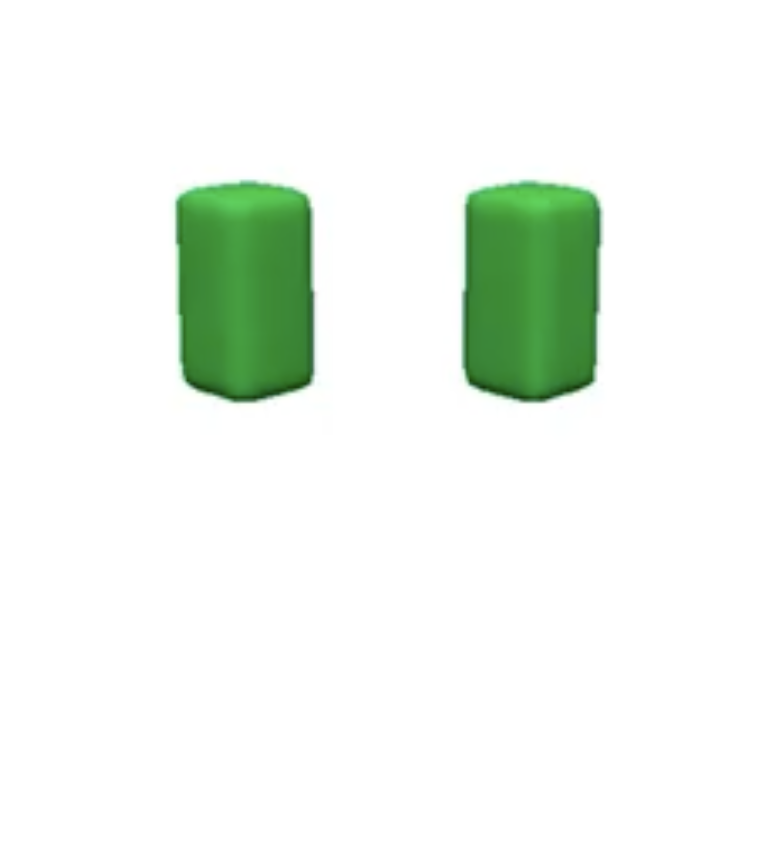
\includegraphics[width=0.4\linewidth]{../project_demos/fg1.png}
  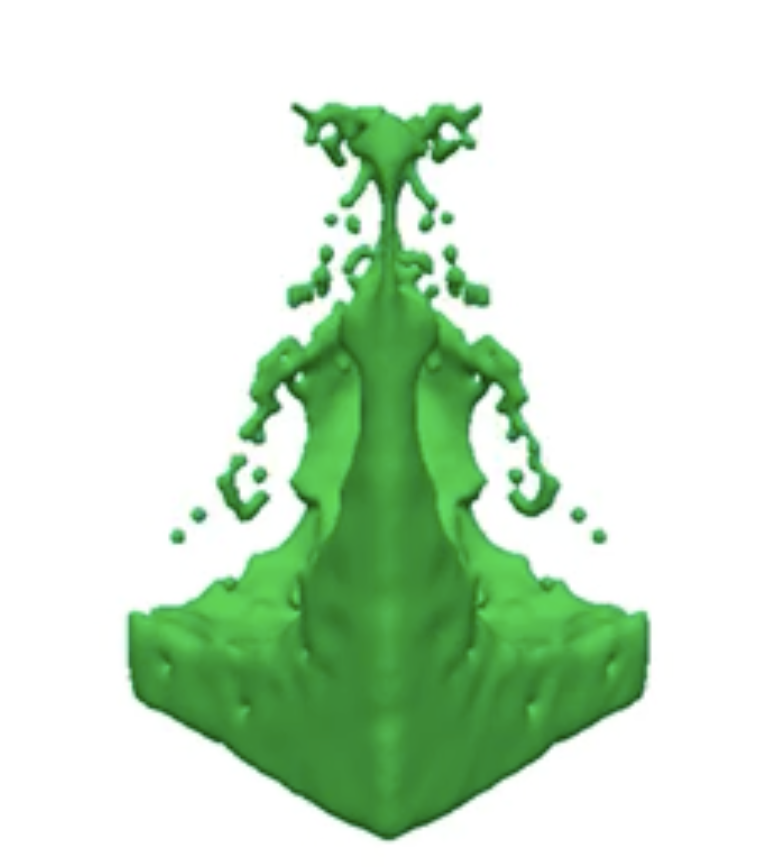
\includegraphics[width=0.4\linewidth]{../project_demos/fg2.png}
  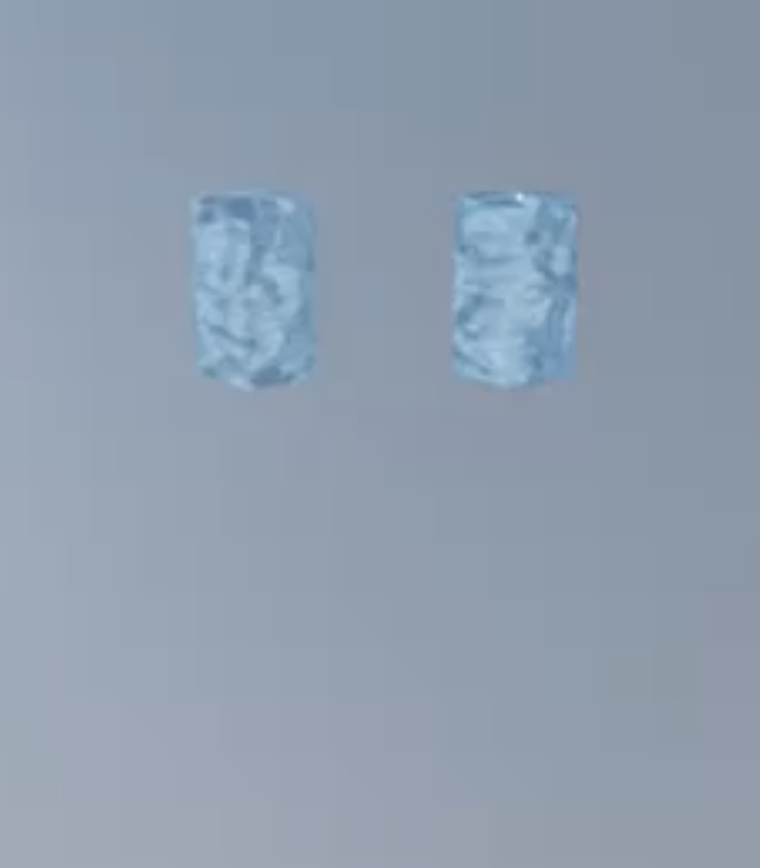
\includegraphics[width=0.4\linewidth]{../project_demos/fb1.png}
  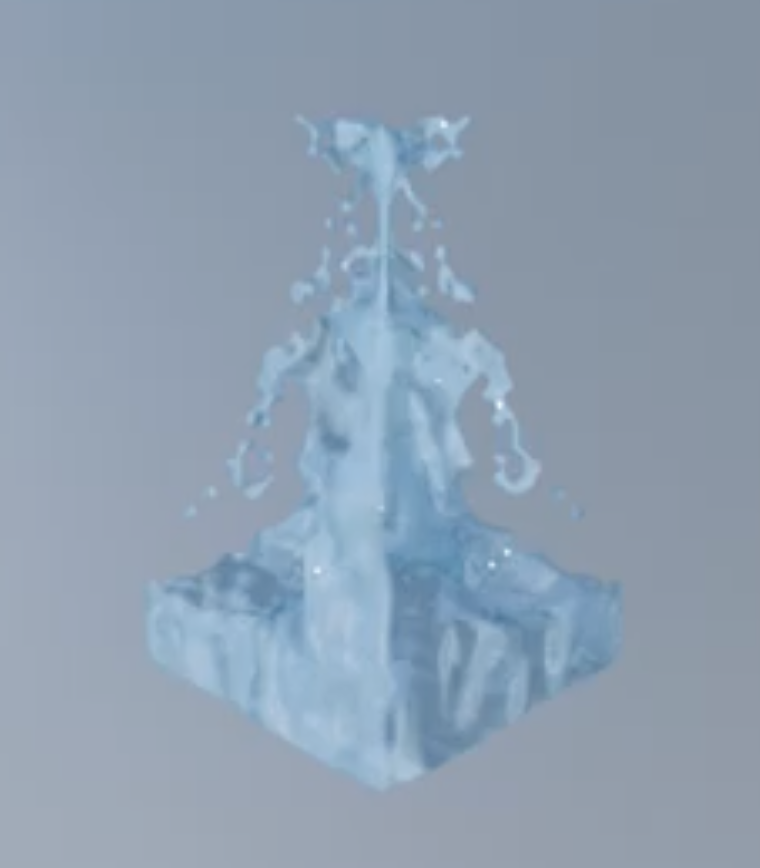
\includegraphics[width=0.4\linewidth]{../project_demos/fb2.png}
  \caption{Fluid simulation. Top: OpenGL; Bottom: Blender. Left: The fluid is initialized in two cuboids; Right: The scene after $1.5$ seconds.}
  \label{fig-fluid}
\end{figure}

\subsection{Cloth Simulation}

We simulate a cloth with $200\times 200$ particles, as shown in Figure \ref{fig-cloth}.

\begin{figure}[h]
  \centering
  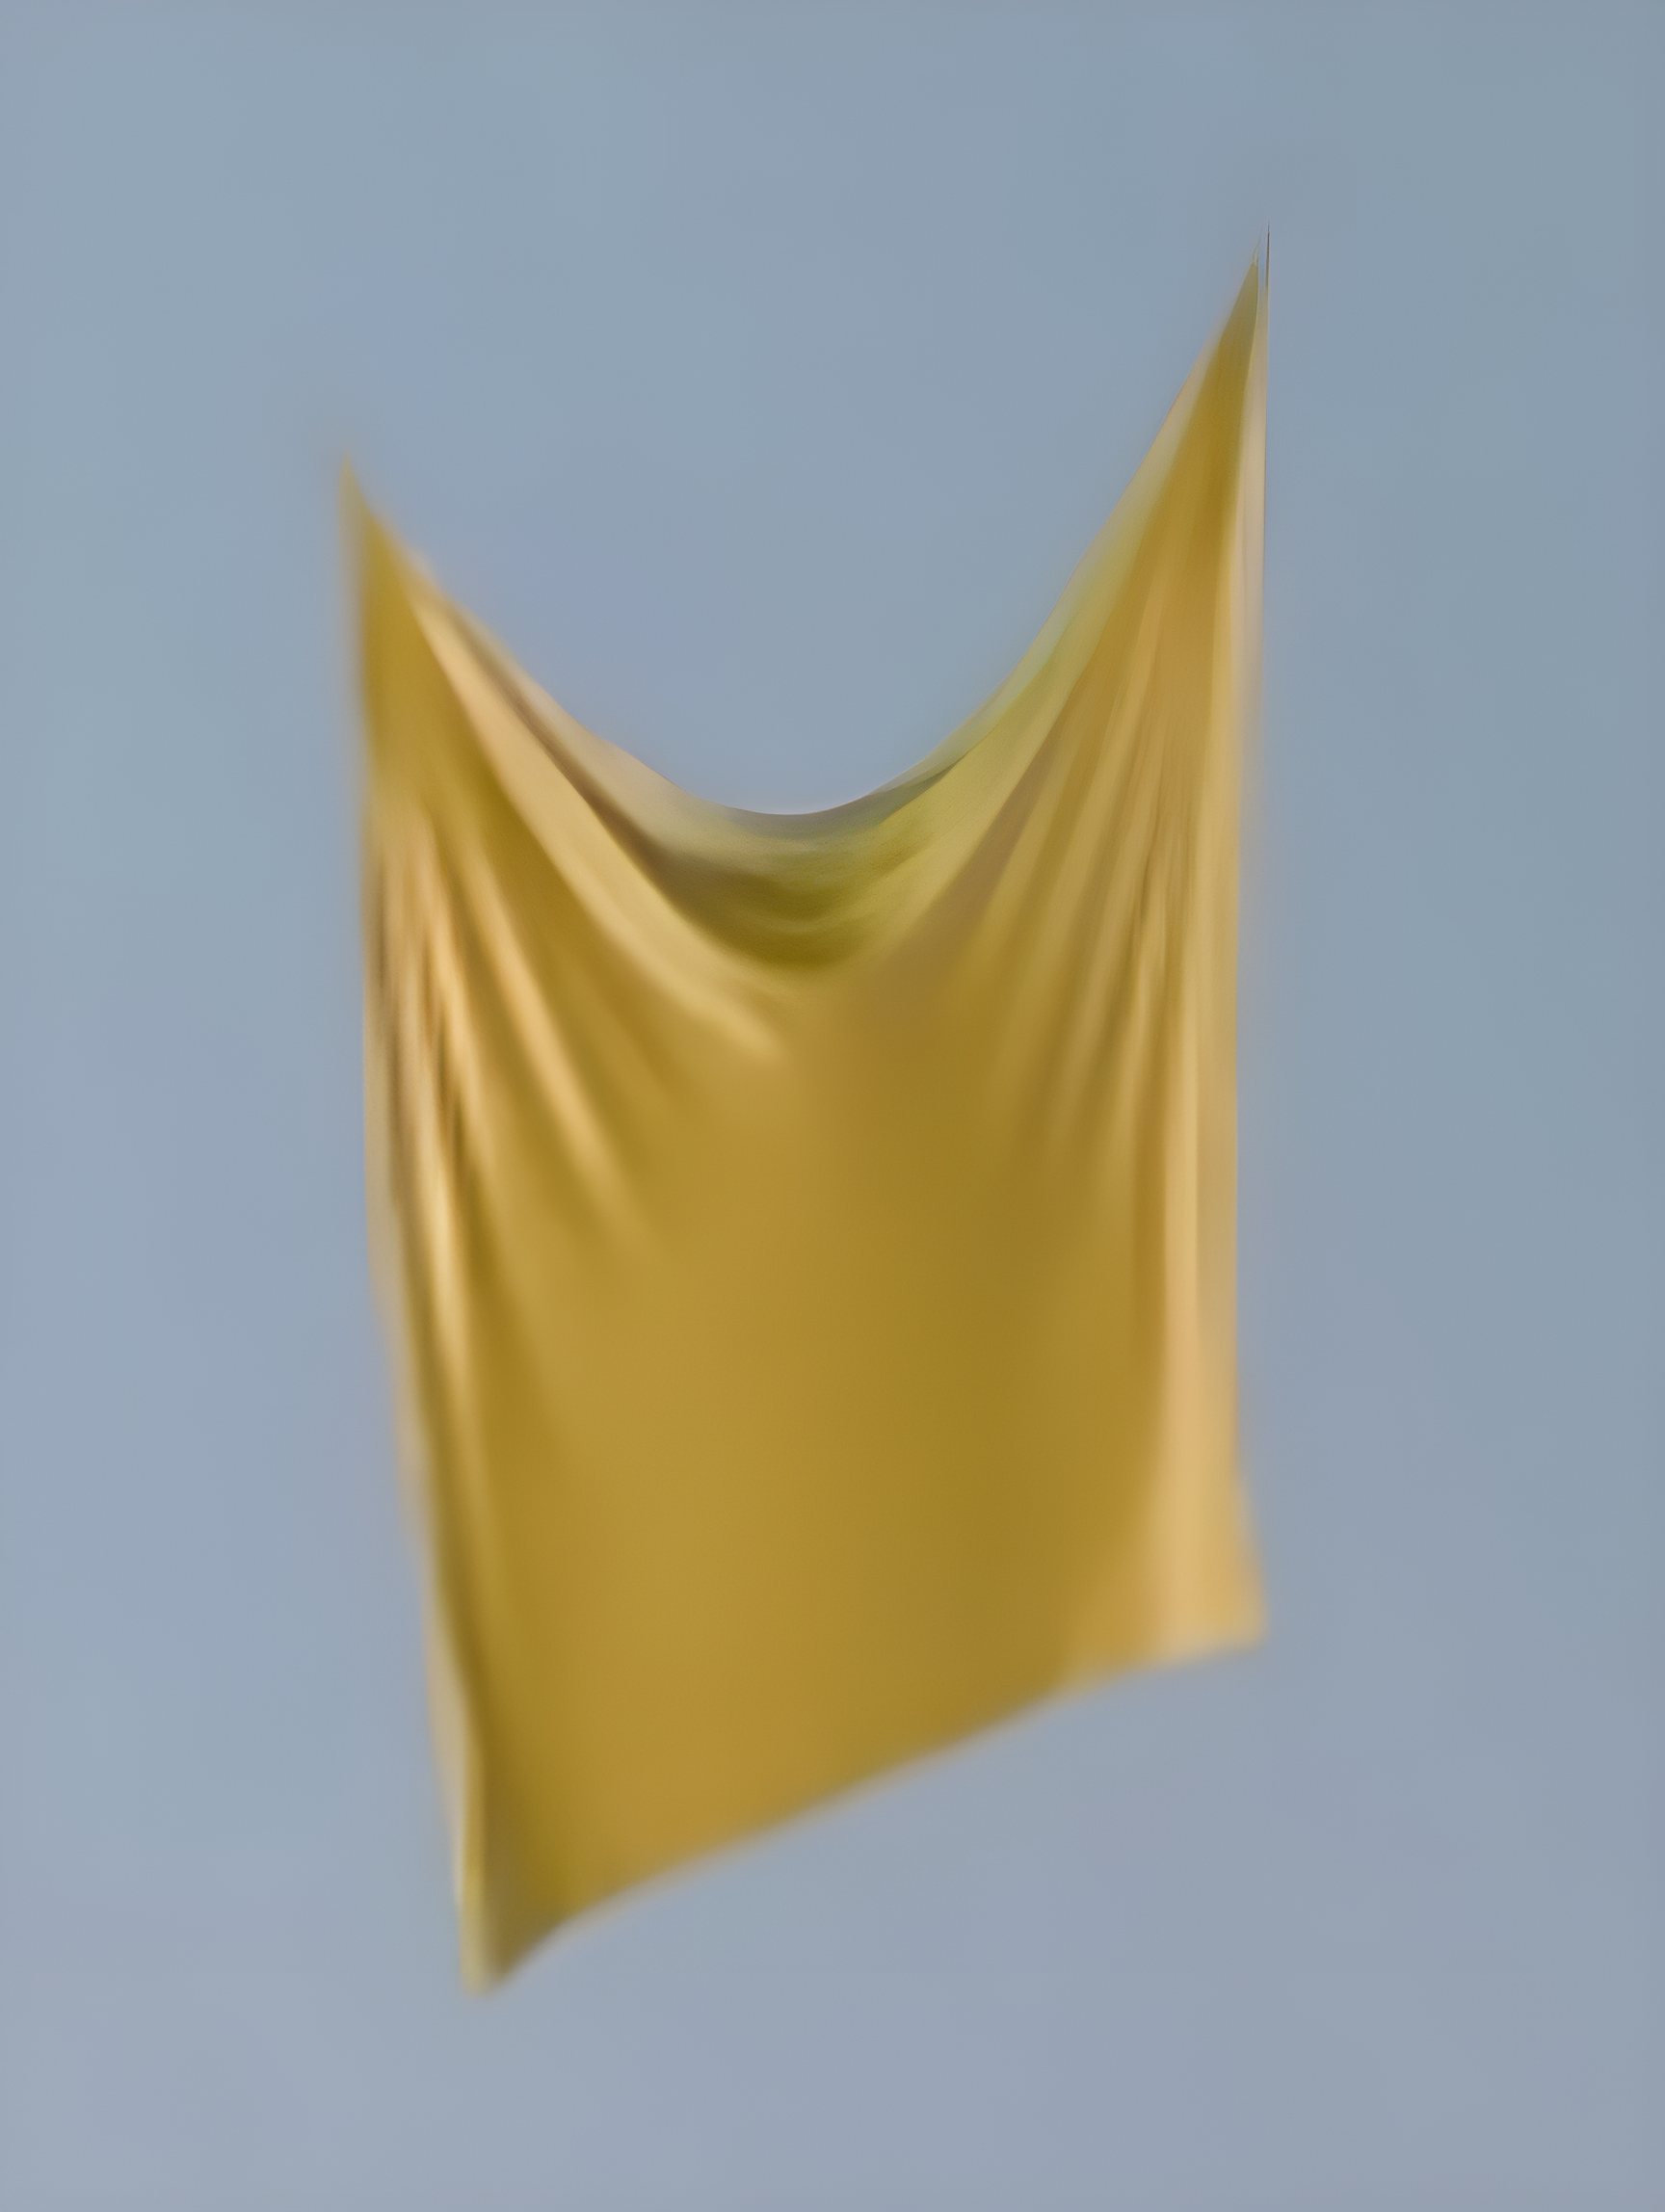
\includegraphics[width=0.4\linewidth]{../project_demos/cloth.png}
  \caption{Cloth simulation}
  \label{fig-cloth}
\end{figure}

We can see that the texture of the cloth is very realistic, and does not penetrate itself on the top. Note that, we can change the damping constant $k_{\text{damping}}$ to control the cloth's behavior, as shown in Figure \ref{fig-cloth-damping}.

\begin{figure}[h]
  \centering
  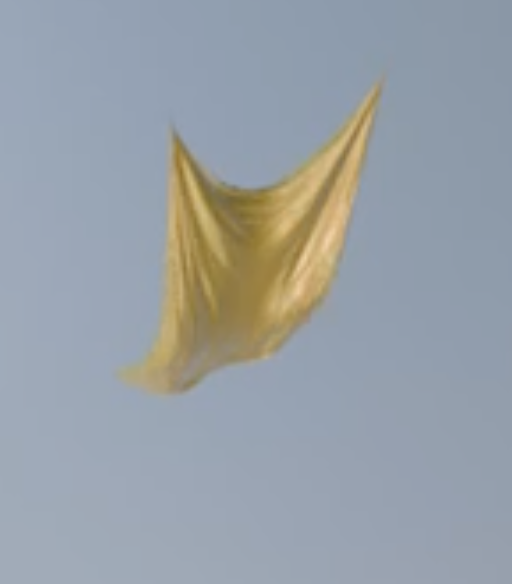
\includegraphics[width=0.25\linewidth]{../project_demos/cloth2.png}
  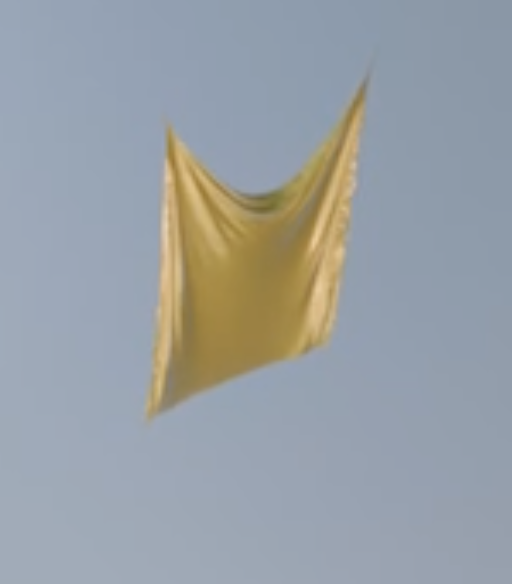
\includegraphics[width=0.25\linewidth]{../project_demos/cloth4.png}
  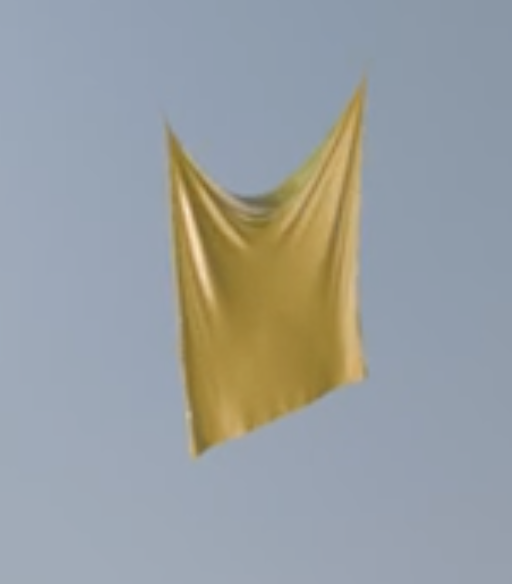
\includegraphics[width=0.25\linewidth]{../project_demos/cloth6.png}
  \caption{Cloth simulation with different damping constants (at $t=5.5$). Left: $k_{\text{damping}}=2\times 10^{-4}$; Middle: $k_{\text{damping}}=4\times 10^{-4}$; Right: $k_{\text{damping}}=6\times 10^{-4}$.}
  \label{fig-cloth-damping}
\end{figure}

We also simulate a cloth with a sphere, as shown in Figure \ref{fig-cloth-sphere}, with cloth resolution $200\times 200$ as well. The XPBD method enables the cloth to adjust its texture smoothly.

\begin{figure}[h]
  \centering
  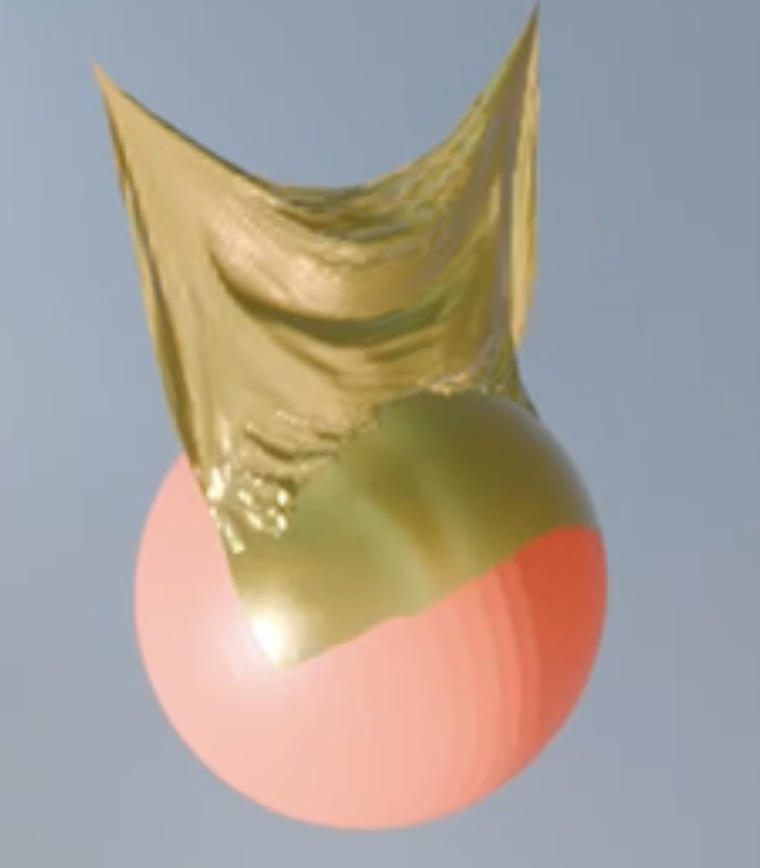
\includegraphics[width=0.25\linewidth]{../project_demos/sfcoup.png}
  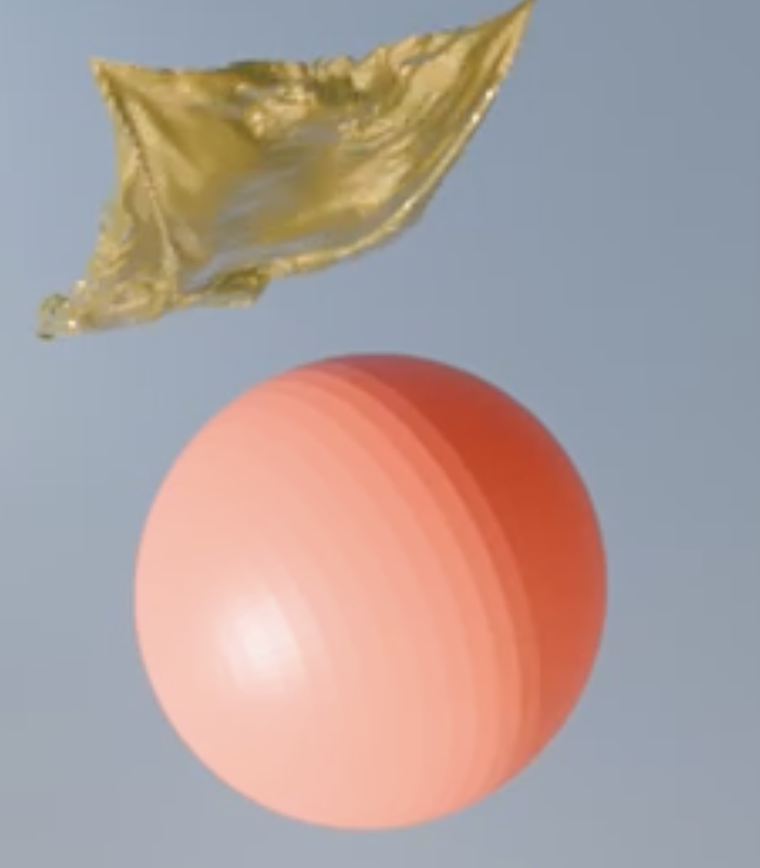
\includegraphics[width=0.25\linewidth]{../project_demos/sfcoup2.png}
  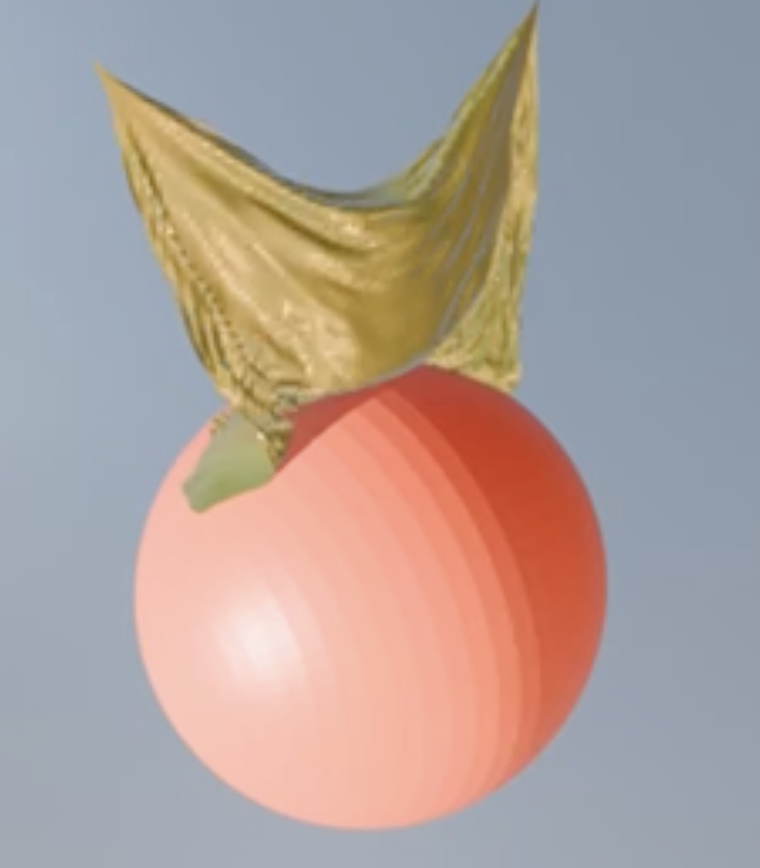
\includegraphics[width=0.25\linewidth]{../project_demos/sfcoup3.png}
  \caption{Cloth collide with sphere; three sequential frames.}
  \label{fig-cloth-sphere}
\end{figure}

\subsection{Cloth-fluid coupling}

We simulate a cloth-fluid coupling system, as shown in Figure \ref{fig-coup}. The resolution of fluid and cloth is $20\times 40\times 20$ and $80\times 80$, respectively.

As we have introduced above, we can adjust the value of $\eta$ to control the penetrating ratio of the fluid. If $\eta$ is large, as shown in the left, no penetration will be detected; on the other hand, when $\eta$ is small, as shown in the right, half of the fluid particles penetrate and cloth and half of them is blocked back, providing different visual effect.
\begin{figure}[h]
  \centering
  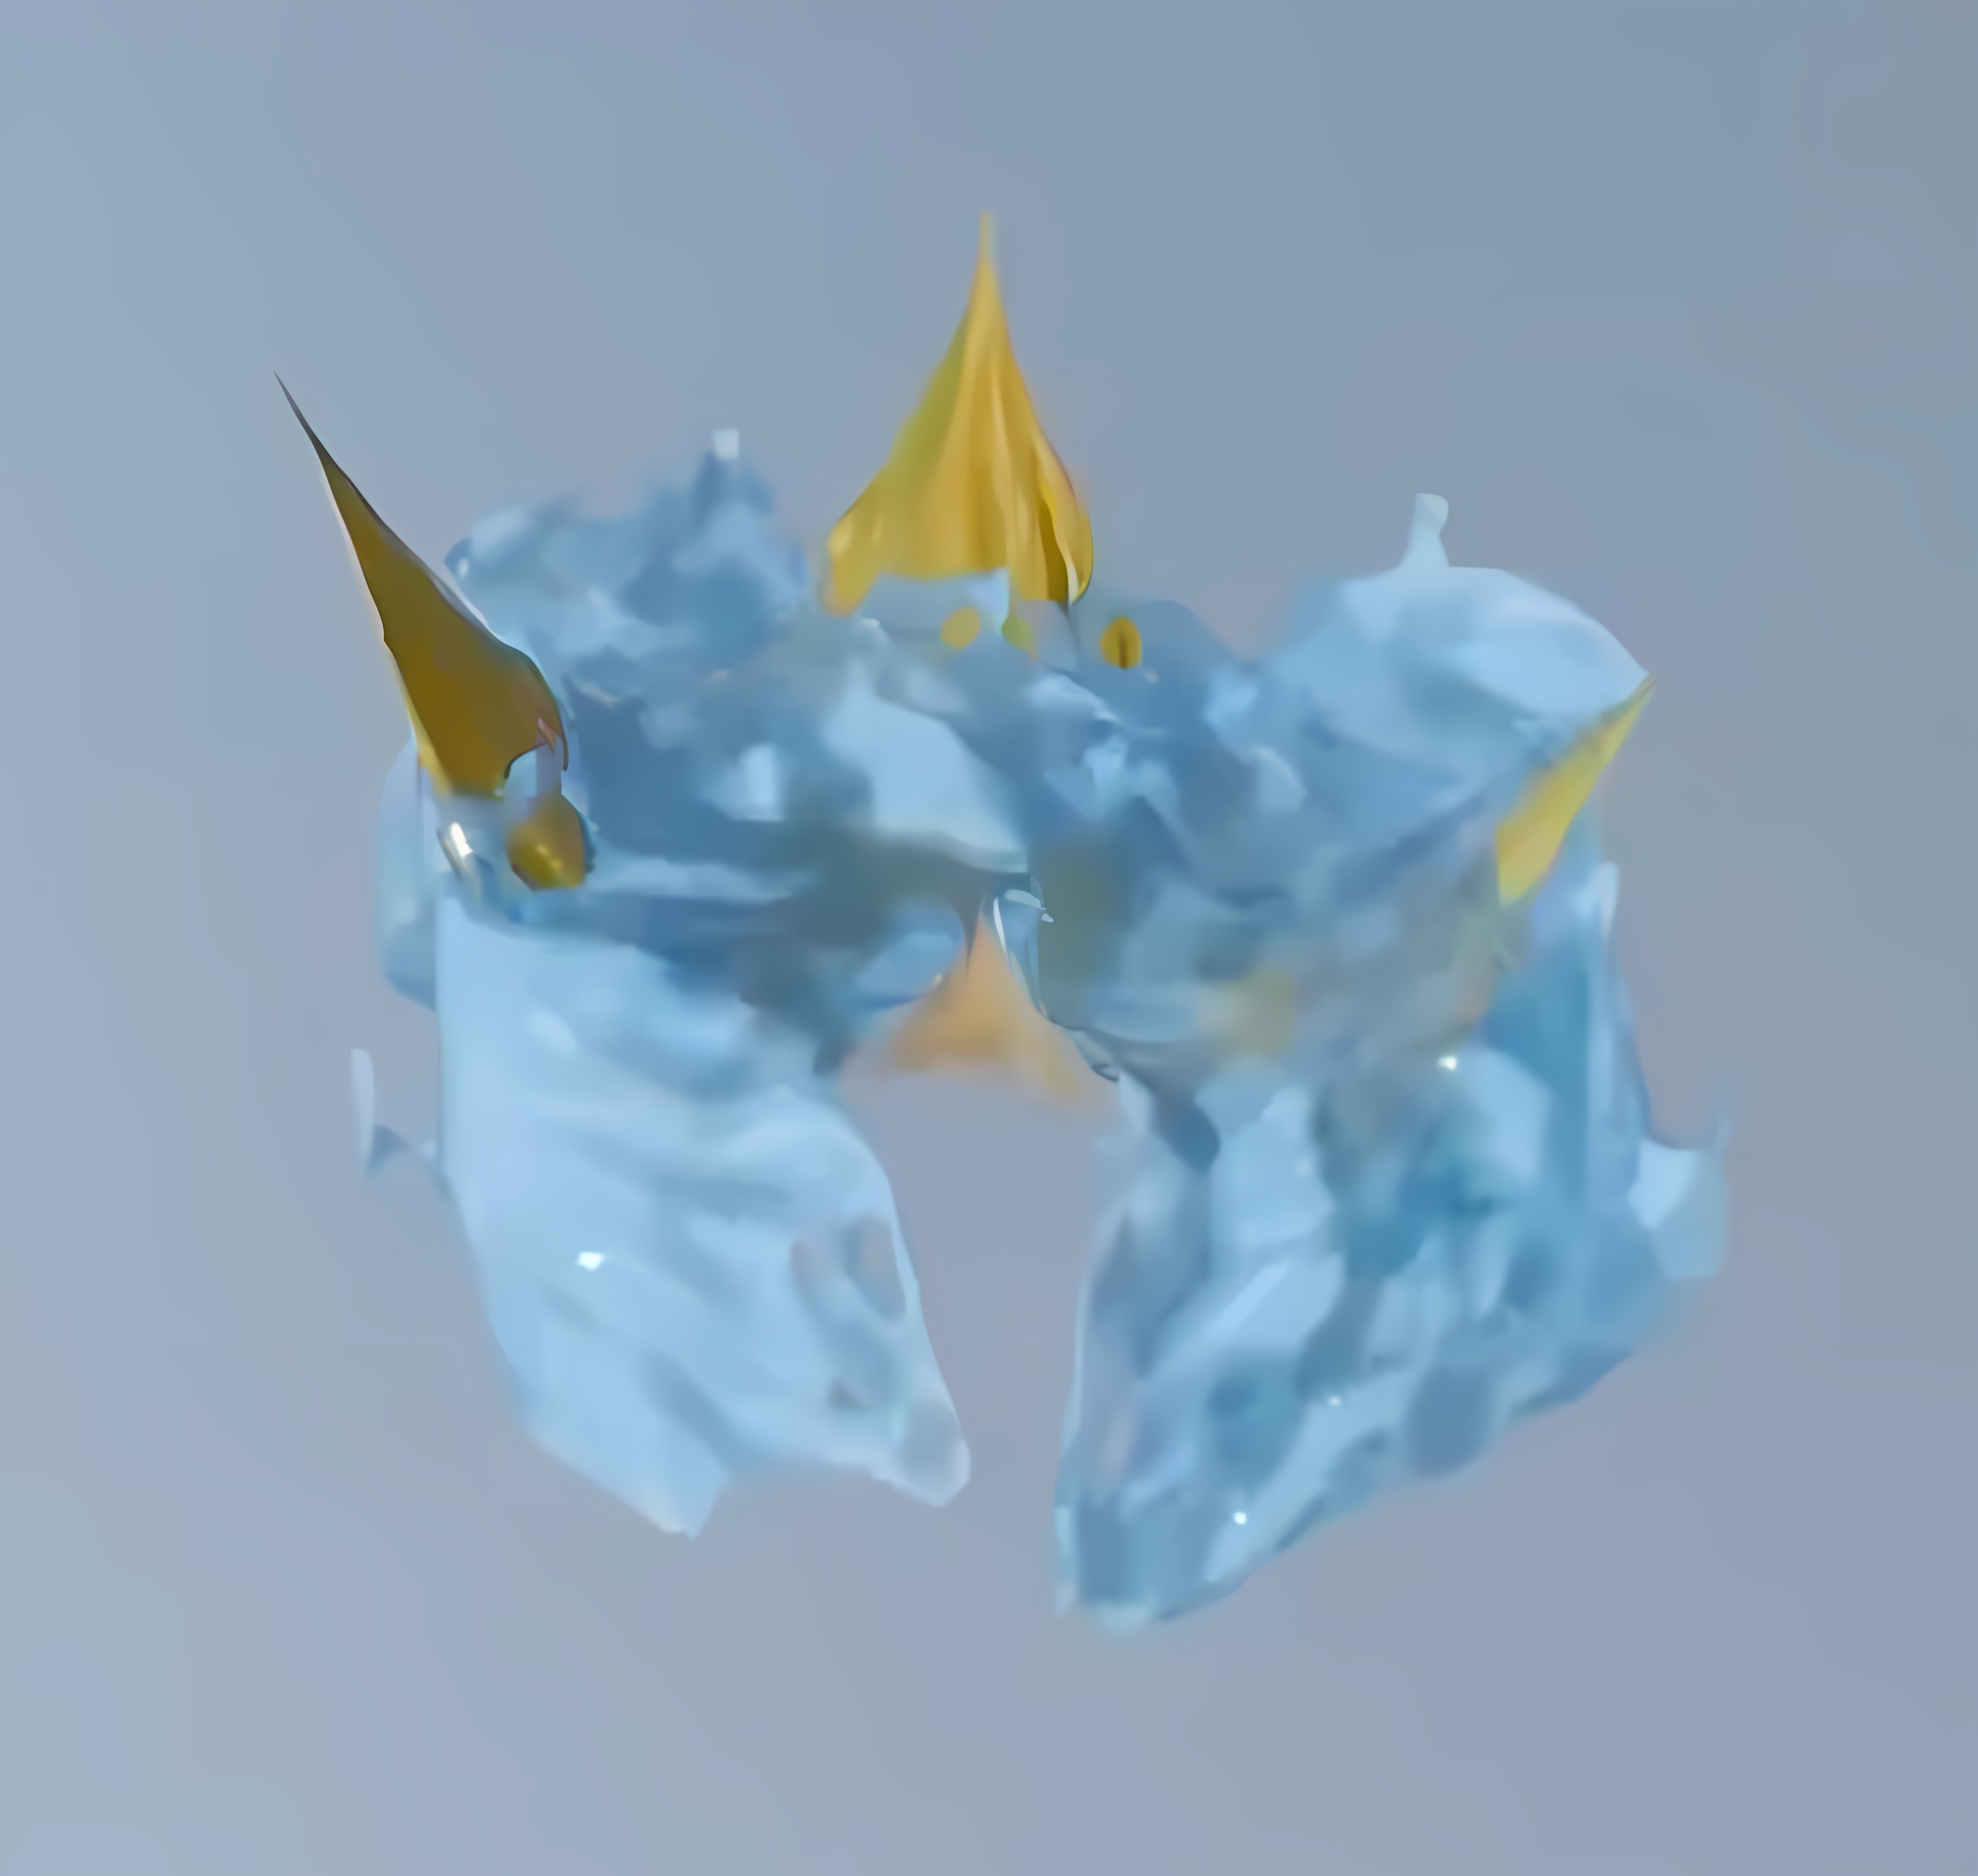
\includegraphics[width=0.4\linewidth]{../project_demos/coup1.png}
  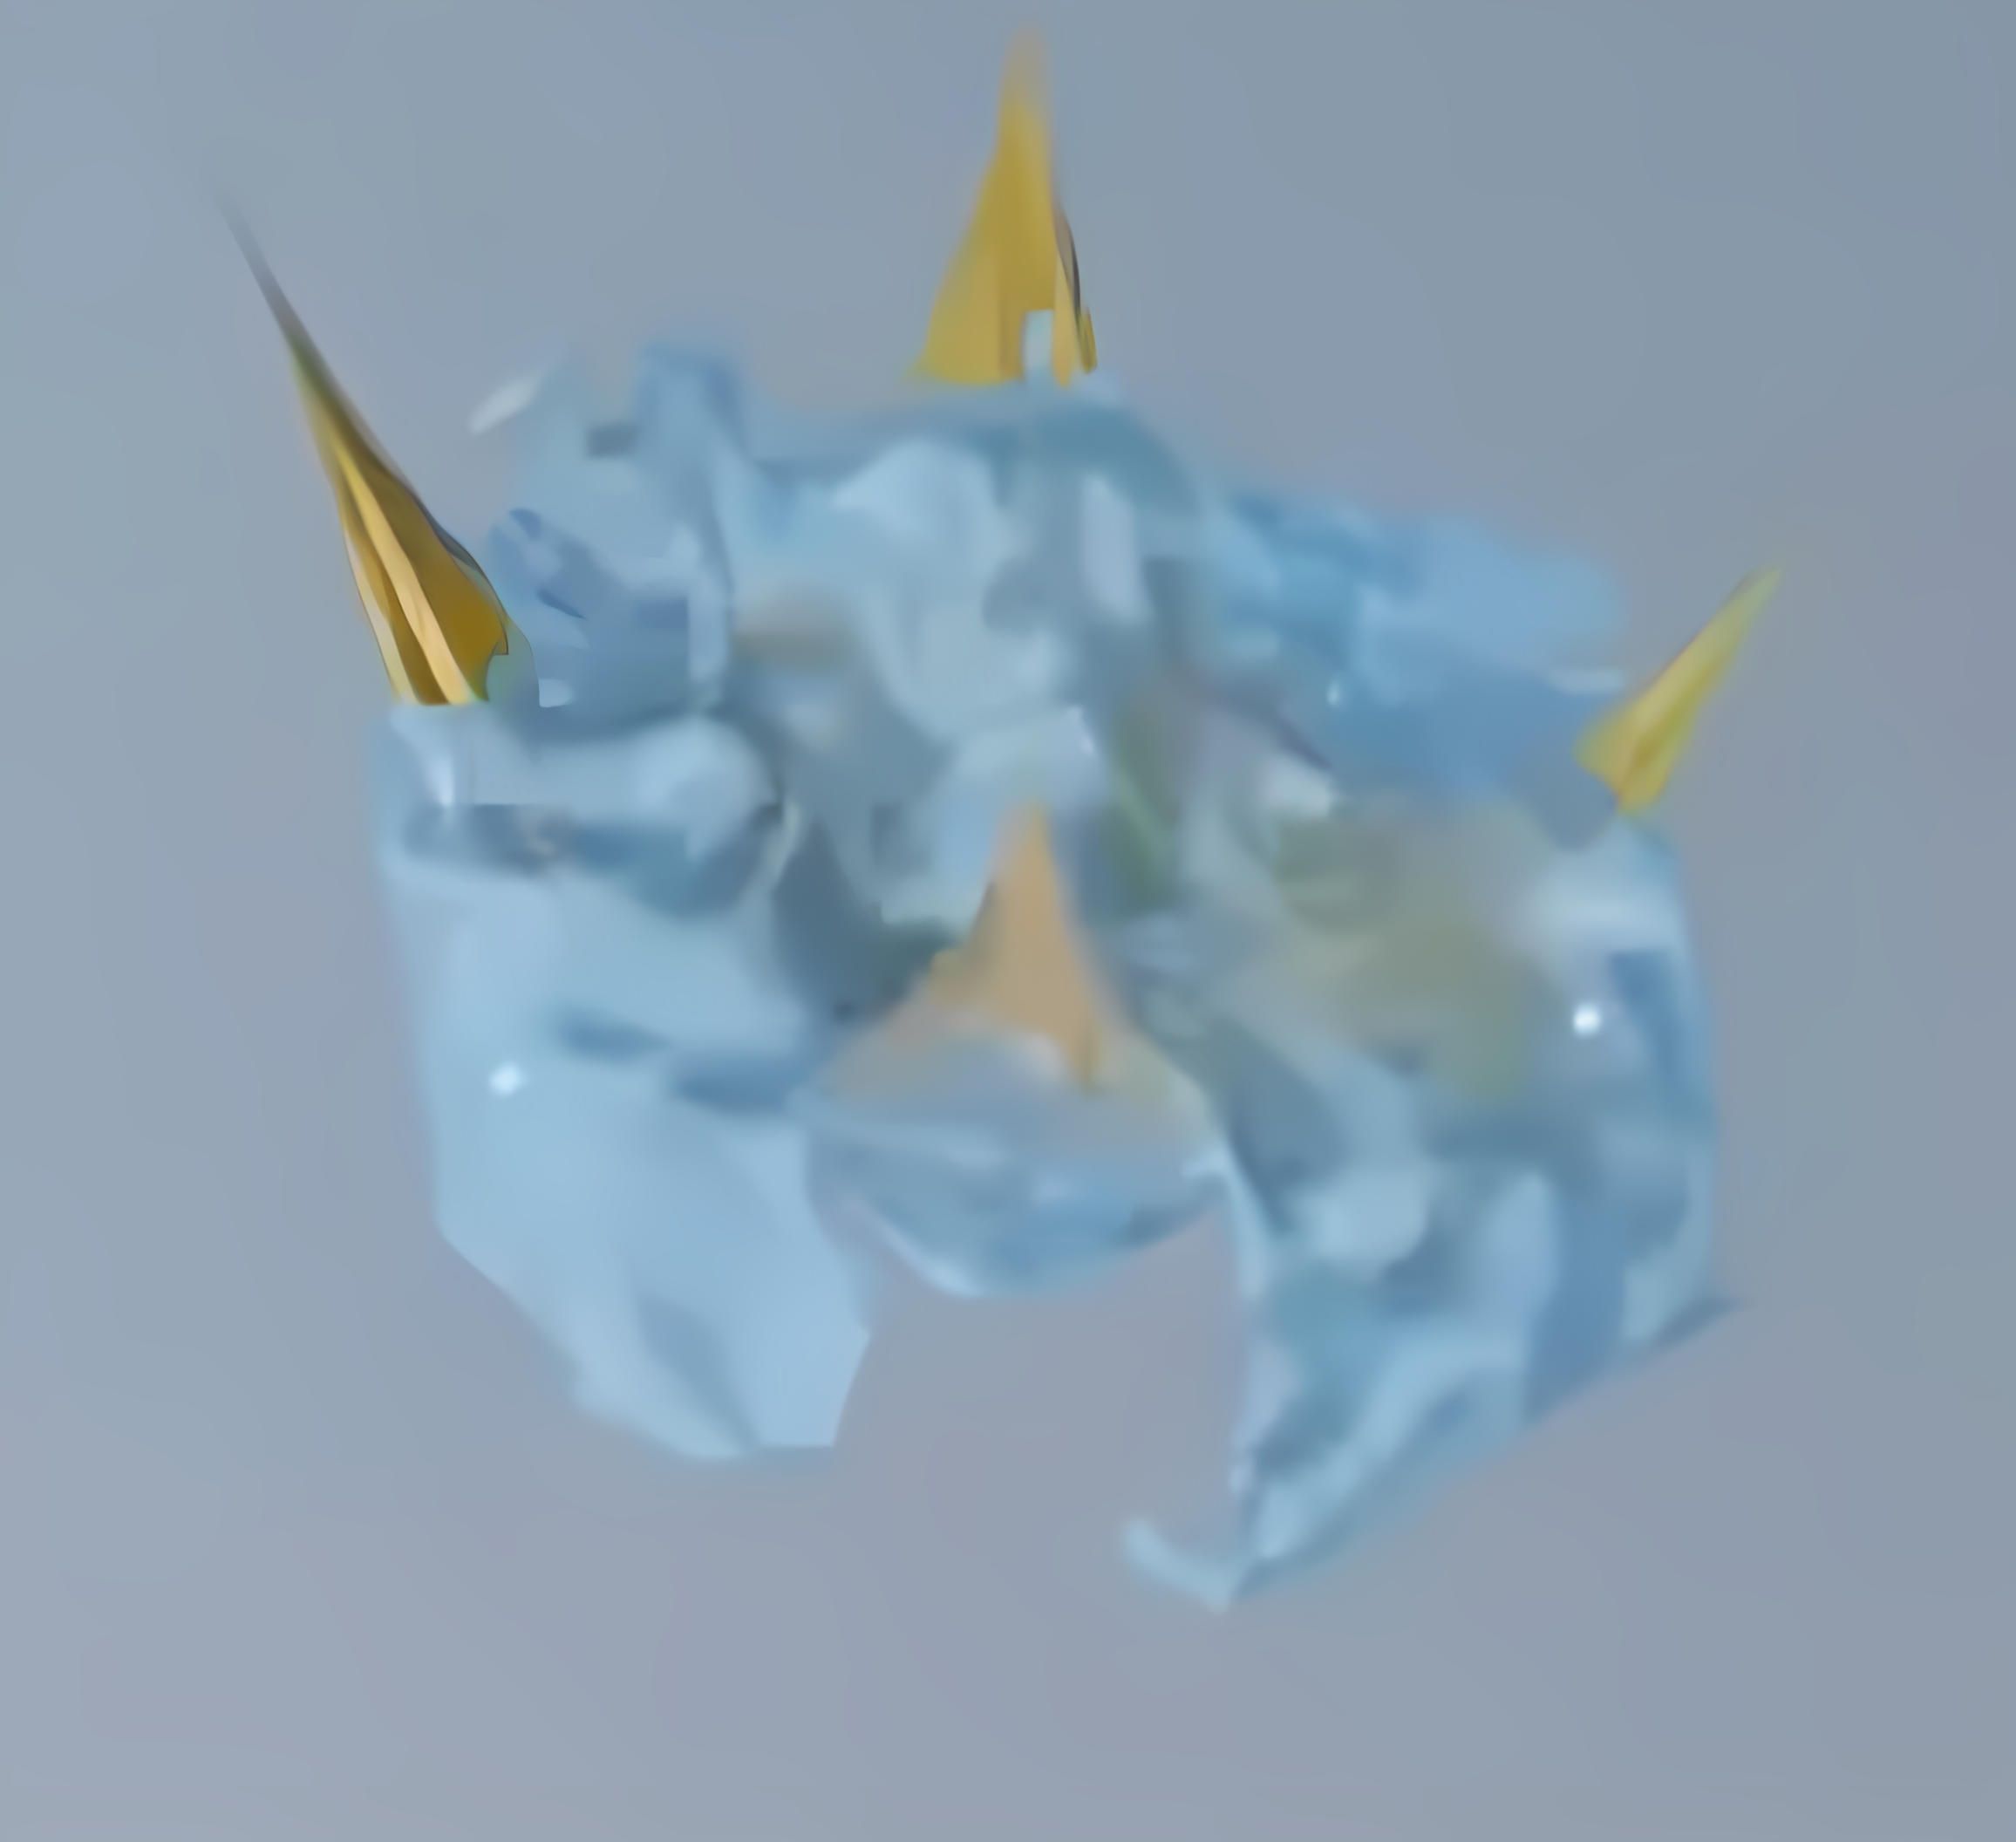
\includegraphics[width=0.415\linewidth]{../project_demos/coup2.png}
  \caption{Cloth-fluid coupling. Left: $\eta=0.05$; Right: $\eta=0.03$.}
  \label{fig-coup}
\end{figure}

\section{External Tools}

We only used the following external tools, and the only funtionality we used is listed below:

\begin{itemize}
\item \textbf{glm}: to handle matrix operations.
\item \textbf{OpenGL}: to render the simulation results and provide GUI.
\item \textbf{OpenCV}: to generate videos.
\item \textbf{stb\_image\_write}: to save images.
\item \textbf{splashsurf}: to smooth the fluid surface and finalize surface reconstruction.
\item \textbf{Blender (Python)}: to do rendering.
\end{itemize}

\section{Future Plan}

We decided to implement the following features in the future:

\begin{itemize}
\item Refine the coupling method to improve the stability and efficiency.
\item A \textbf{control interface} to interpolate the simulation parameters and change the cloth's position in real-time.
\item The \textbf{wetting effect} of the cloth.
\item More \textbf{constraints} to simulate more complex cloth behaviors, such as collision with rigid bodies.
\end{itemize}

\bibliographystyle{ACM-Reference-Format}
\bibliography{midterm_report_reference}